\documentclass{article}
\usepackage {inputenc, fullpage, listings, amsmath, graphicx, amssymb, xcolor}

\parindent 0pt

\title{%
   ECE 260: Continuous-Time Signals and Systems\\
    \Large Alex Holland - A01\\
    Assignment 1\\
    }
\date{}

\begin{document}

\maketitle


A.1 (c) {\bf [convert to cartesian form]}\\

\begin{equation*}
\begin{split}
     z &= 2e^{j7\pi/6}\\
     z &= x+jy\\
     x &= 2cos\frac{7\pi}{6}, y = 2sin\frac{7\pi}{6}\\
     z &= -\sqrt{3}-j\\
    \end{split}
\end{equation*} 
 
A.2 (b) {\bf [convert to polar form, principal argument]}\\
  
\begin{equation*}
\begin{split}
    & \frac{-1}{2} - j \frac{\sqrt{3}}{2}\\
    |z| &= \sqrt{x^2+y^2}\\
    |z| &= \sqrt{(-\frac{1}{2})^2(\frac{\sqrt{3}}{2})^2} = 1\\
    argz = arctan&(\frac{-\frac{\sqrt{3}}{2}}{-\frac{1}{2}}) + \pi = \frac{\pi}{3} + \pi = \frac{4\pi}{3}\\
    z &= 1e^{j4\pi/3}\\
\end{split}
\end{equation*} 

\begin{center}
    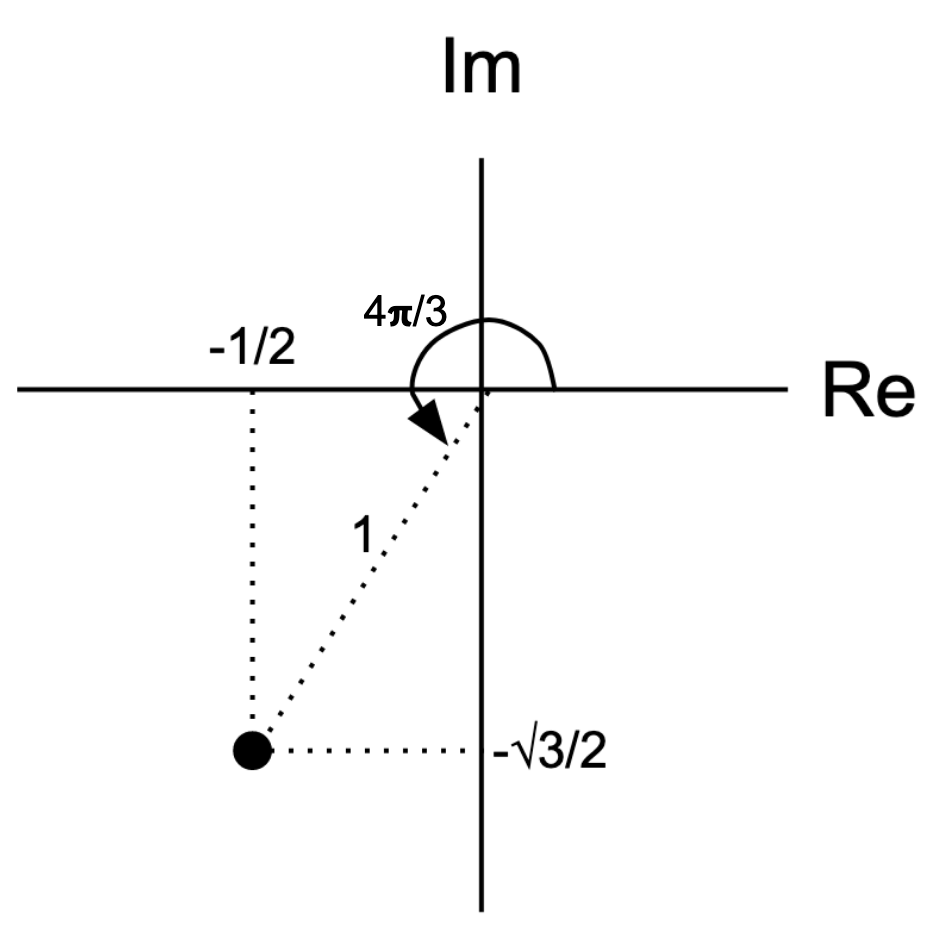
\includegraphics[width=0.25\textwidth]{a2b.png}
\end{center}

A.2 (d)

\begin{equation*}
\begin{split}
    & 1 + j\sqrt{3}\\
    |z| &= \sqrt{x^2+y^2}\\
    |z| &= \sqrt{(1)^2+(\sqrt{3})^2} = 2\\
    argz &= arctan(\frac{\sqrt{3}}{1}) = \frac{\pi}{3}\\
    z &= 2e^{j\pi/3}
\end{split}
\end{equation*} 

\begin{center}
    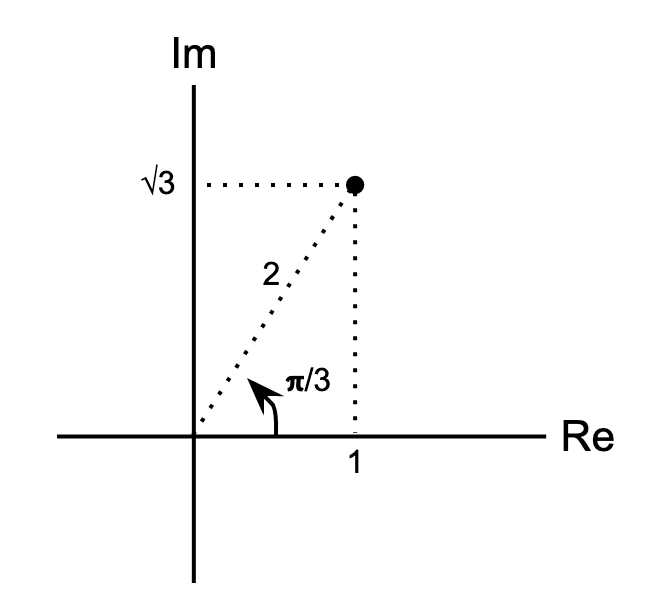
\includegraphics[width=0.3\textwidth]{a2d.png}
\end{center}

A.3 (a){\bf [complex arithmetic]}\\

\begin{equation*}
\begin{split}
    & 2(\frac{\sqrt{3}}{2}-j\frac{1}{2})+j(\frac{1}{\sqrt{2}}e^{j(-3\pi/4)}) \text{ in Cartesian form}\\
    & = \sqrt{3} - j + j (\frac{1}{\sqrt{2}}cos(\frac{-3\pi}{4}) + j \frac{1}{\sqrt{2}} sin(\frac{-3\pi}{4}))\\
    & = \sqrt{3} - j + j((\frac{1}{\sqrt{2}})(\frac{-\sqrt{2}}{2}) + j(\frac{1}{\sqrt{2}})(\frac{-\sqrt{2}}{2}))\\
    & = \sqrt{3} - j + j(-\frac{1}{2} - \frac{1}{2}j)\\
    & = \sqrt{3} - j - \frac{1}{2}j + \frac{1}{2}\\
    & = \frac{2 \sqrt{3} + 1}{2} - j\frac{3}{2}\\
\end{split}
\end{equation*} 

(b)

\begin{equation*}
\begin{split}
    & (\frac{\sqrt{3}}{2}-j\frac{1}{2}) + j(\frac{1}{\sqrt{2}}e^{j(-3\pi/4)}) \text{ in polar form}\\\\
    & |z| = \sqrt{x^2+y2}\\ 
    & |z| = \sqrt{(\frac{\sqrt{3}}{2})^2+(\frac{1}{2})^2} = 1\\
    & argz = arctan(\frac{-1/2}{\sqrt{3}/2}) = -\frac{\pi}{6}\\\\
    (\frac{\sqrt{3}}{2}-j\frac{1}{2}) + j(\frac{1}{\sqrt{2}}e^{j(-3\pi/4)}) &= (1e^{j(-\pi/6)}) (\frac{1}{\sqrt{2}}e^{j(-3\pi/4)})\\
    &= \frac{1}{\sqrt{2}} e^{j(\frac{-\pi}{6} + \frac{-3\pi}{4})}\\
    &= \frac{1}{\sqrt{2}}e^{j(-11\pi/12)}
\end{split}
\end{equation*} 

(f)

\begin{equation*}
\begin{split}
    & (1+j)^{10} \text{ in cartesian form}\\\\
    & |z| = \sqrt{x^2+y2}\\ 
    & |z| = \sqrt{1^2 + 1^2} = \sqrt{2}\\
    & argz = arctan(\frac{1}{1}) = \frac{\pi}{4}\\\\
    (1+j)^{10} &= [\sqrt{2}cos(\frac{\pi}{4}) + \sqrt{2}jsin(\frac{\pi}{4})]^{10}\\
    &= (\sqrt{2})^{10}[cos(\frac{\pi}{4}(10) + jsin(\frac{\pi}{4}(10)))]\\
    &= 32[0+j]\\
    &= 32j
\end{split}
\end{equation*} 

(g)

\begin{equation*}
\begin{split}
    &= \frac{1+j}{1-j} \text{ in polar form}\\
    & |z| = \sqrt{x^2+y2}\\ 
    & |z| = \sqrt{1^2 + 1^2} = \sqrt{2}\\
    & argz = arctan(\frac{1}{1}) = \frac{\pi}{4}\\\\
    & argz = arctan(\frac{-1}{1}) = \frac{-\pi}{4}\\\\
    \frac{1+j}{1-j} &= \frac{\sqrt{2}e^{j(\pi/4)}}{\sqrt{2}e^{j(-\pi/4)}}\\
    &= e^{j(\frac{\pi}{4}-(-\frac{\pi}{4}))} \\
    &= e^{j\frac{\pi}{2}}\\
\end{split}
\end{equation*} 

A.4 (b) {\bf [properties of complex numbers]}\\

\begin{equation*}
\begin{split}
   arg(\frac{z_1}{z_2}) &= arg_{z_1} - arg_{z_2}, \text{ for } z \neq 0\\
   & \text{let } z_1 = r_1e^{j\theta_1}\\
   & \text{let } z_2 = r_2e^{j\theta_2}\\
   & \frac{z_1}{z_2} = \frac{r_1e^{j\theta_1}}{r_2e^{j\theta_2}}\\
   &= \frac{r_1}{r_2}e^{j(\theta_1-\theta_2)}\\
   & arg(\frac{z_1}{z_2}) = \theta_1 - \theta_2\\
   &= argz_1-argz_2\\
\end{split}
\end{equation*} 


(e)
\begin{equation*}
\begin{split}
   (z_1 z_2)^* &= z_1^*z_2^*\\
   \text{let } z_1 &= x_1 + jy_1\\
   \text{let } z_2 &= x_2 + jy_2\\\\
   (z_1z_2) &= (x_1 + jy_1)(x_2 + jy_2)\\
   &= (x_1x_2 + jx_1y_2 + jx_2y_1 - y_1y_2)\\
   &= (x_1x_2 = y_1y_2) + j(x_1y_2 + x_2y_1)\\
   (z_1z_2)^* &= (x_1x_2- y_1y_2) - j(x_1y_2 + x_2y_1)\\\\
   z_1^*z_2^* &= (x_1 - jy_1)(x_2 - jy_2)\\
   &= (x_1x_2 - jx_1y_2 - jx_2y_1 - y_1y_2)\\
   &= (x_1x_2 - y_1y_2) - j(x_1y_2 + x_2y_1)\\\\
   & \therefore (z_1z_2)^* = z_1^*z_2^*
\end{split}
\end{equation*} 


A.5 (b) {\bf [Euler's relation]}\\

\begin{equation*}
\begin{split}
    sin\theta &= \frac{1}{-2j}[e^{j\theta}-e^{-j\theta}]\\
    &= \frac{1}{2j}[cos\theta + jsin\theta - (cos\theta - jsin\theta)]\\
    &= \frac{1}{2j}(2jsin\theta)\\
    &= sin\theta\\
\end{split}
\end{equation*}

A.6 (b) {\bf [poles/zeros]}\\

\begin{equation*}
\begin{split}
    r(z) &= z + 3 + 2z^{-1}\\
    &= z + 3 + \frac{2}{z}\\
    r(-1) &= -1 + 3 + \frac{2}{-1}\\
    &= 0\\
    r(-2) &= -2 + 3 + \frac{2}{-2}\\
    &= 0\\
\end{split}
\end{equation*}
first order zeros at $-1$ and $-2$\\
first order pole at $0$\\

\begin{center}
    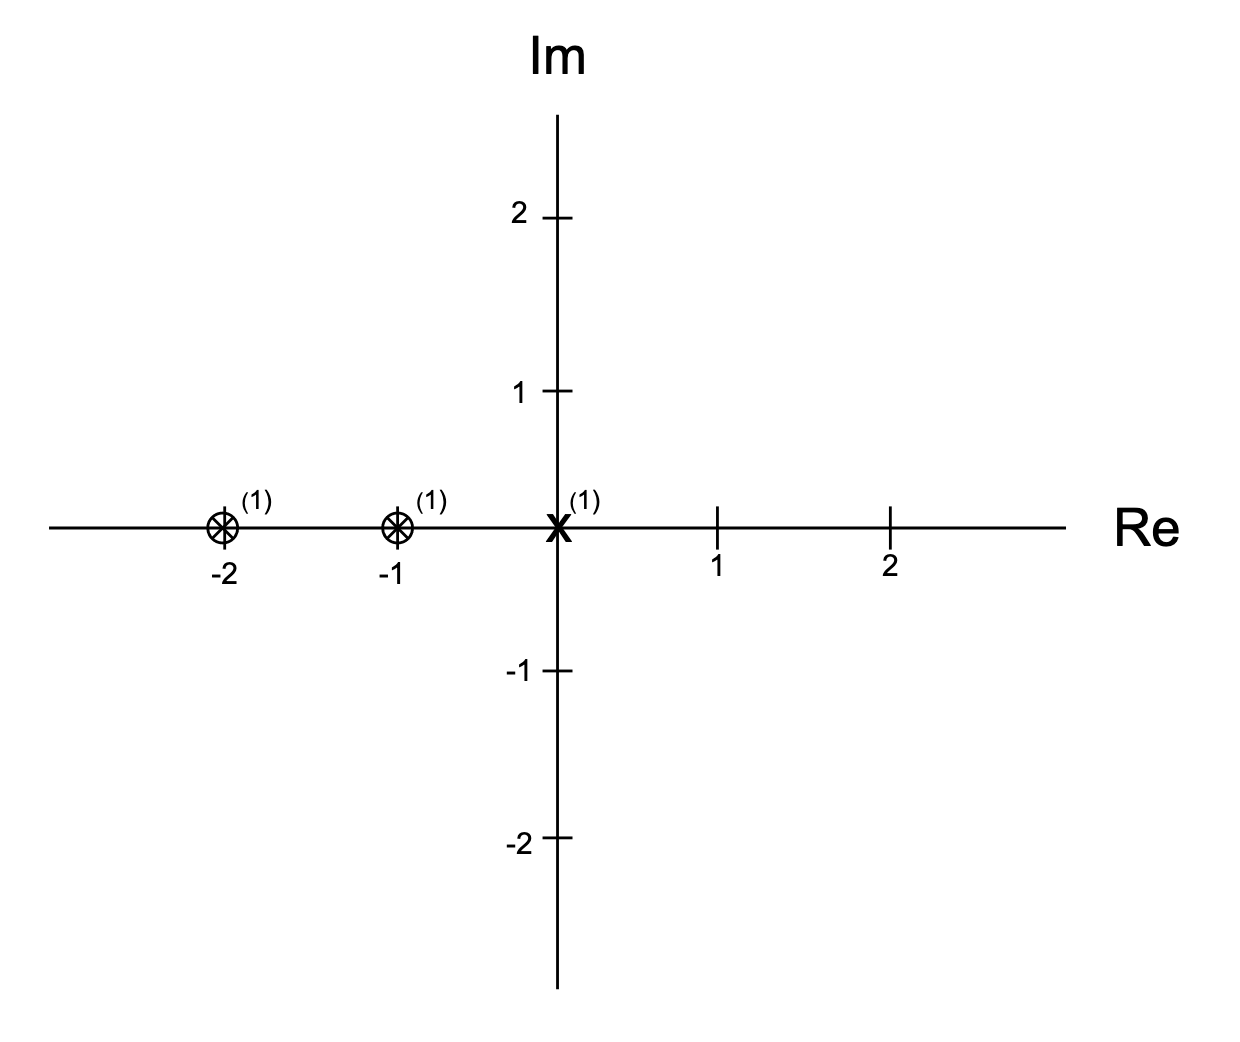
\includegraphics[width=0.5\textwidth]{a6b.png}
\end{center}


(c)
\begin{equation*}
\begin{split}
    F(z) &= \frac{(z^2+2z+5)(z^2+1)}{(z^2+2z+2)(z^2+3z+2)}\\
\end{split}
\end{equation*}
factor the numerator polynomials:
\begin{equation*}
\begin{split}
    z &= \frac{-b \pm \sqrt{b^2 - 4ac}}{2a}\\
    &= \frac{-2 \pm \sqrt{2^2 - 4(1)(5)}}{2(1)}\\
    &= \frac{-2 \pm \sqrt{-16}}{2}\\
    &= -1 \pm 2j\\
    &= \{-1 + 2j, -1-2i\}\\
    &= (z + 1 + 2j)(z + 1 - 2j)\\\\
    z^2+1 &= (z+j)(z-j)\\
\end{split}
\end{equation*}
factor the numerator polynomials:
\begin{equation*}
\begin{split}
    z &= \frac{-b \pm \sqrt{b^2 - 4ac}}{2a}\\
    &= \frac{-2 \pm \sqrt{2^2 - 4(1)(2)}}{2(1)}\\
    &= \frac{-2 \pm \sqrt{-4}}{2}\\
    &= \frac{-2 \pm 2j}{2}\\
    &= -1 \pm j\\
    &= \{-1 + j, -1-j\}\\
    &= (z + 1 + j)(z + 1 - j)\\\\\
    z^2 + 3z + 2 &= (z + 2)(z + 1)
\end{split}
\end{equation*}

\begin{equation*}
\begin{split}
    f(z) = \frac{(z + 1 + 2j)(z + 1 - 2j)(z+j)(z-j)}{(z + 1 + j)(z + 1 - j)(z + 2)(z + 1)}
\end{split}
\end{equation*}

First order zeros at $-1-2j, -1+2j, -j, j$\\
First order poles at $-1-j, -1+j, -2, -1$\\

\begin{center}
    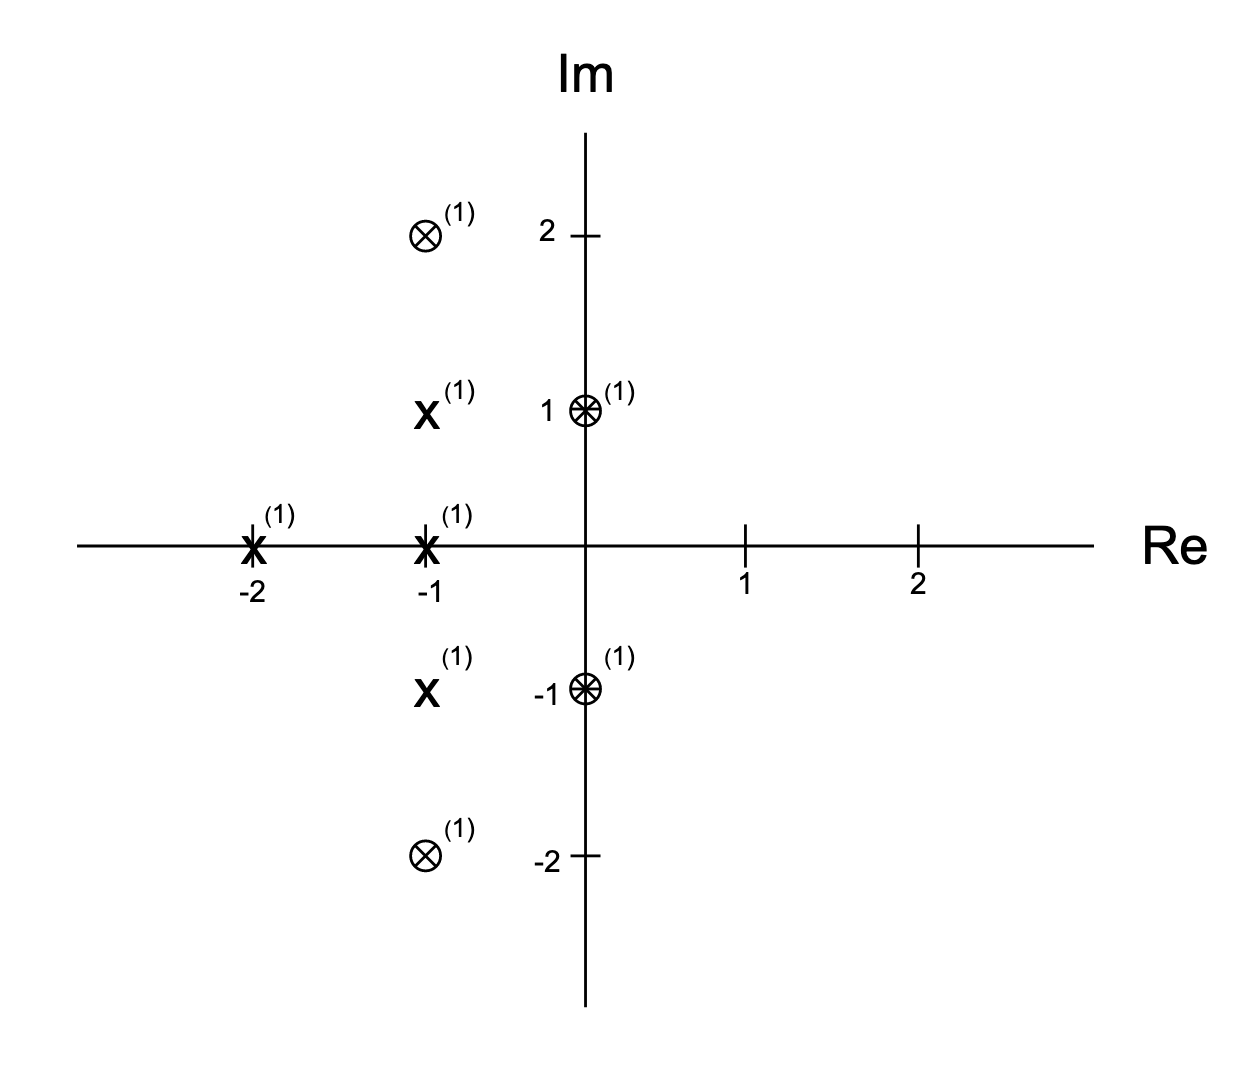
\includegraphics[width=0.5\textwidth]{a6c.png}
\end{center}

A.7 (c) {\bf [continuity, differentiability, analyticity]}\\

\begin{equation*}
\begin{split}
    &\frac{z}{z^4-16}\\
    &= \frac{z}{(z^4 + 4)(z + 2)(z - 2)}
\end{split}
\end{equation*}
{\bf i)} $f(z)$ is continuous everywhere except at $z = \pm 2, \pm 2j$. This is because the denominator goes to zero at these points.\\\\
{\bf ii)} 
\begin{equation*}
\begin{split}
    f'(z) &= \frac{\frac{d}{dz}(z) \cdot (z^4 - 16) - z \cdot \frac{d}{dz}[z^4 - 16]}{(z^4 -16)^2}\\
    &= \frac{z^4 - 16 - z(4z^3)}{(z^4 - 16)^2}\\
    &= \frac{-3x^4 - 16}{(z^4 - 16)^2}
\end{split}
\end{equation*}
$Ff(z)$ is differentiable everywhere except at $z = \pm2, \pm2j$. This is because the denominator goes to zero at these points.\\\\

{\bf iii)} $f(z)$ is analytic everywhere except at $z = \pm 2, \pm 2j$. This is because the denominator goes to zero at these points.\\\\

(d)
\begin{equation*}
\begin{split}
    f'(z) &= z + 2 + z^{-1}\\
    &= z + 2 + \frac{1}{2}
\end{split}
\end{equation*}
{\bf i)} $f(z)$ is continuous everywhere except at $z = 0$. This is because the denominator goes to zero at that point.\\\\

{\bf ii)} 
\begin{equation*}
\begin{split}
    f'(z) &= \frac{d}{dz}(z) + \frac{d}{dz}(2) + \frac{d}{dz}(z^{-1})\\
    &= 1 + (- \frac{1}{z^2})\\
    &= 1 - \frac{1}{z^2}
\end{split}
\end{equation*}
$f(z)$ is differentiable everhwere except at $z = 0$. This is because the denominator goes to zero at that point.\\\\

{\bf iii)} $f(z)$ is analytic everywhere except at $z = 0$. This is because the denominator goes to zero at that point.\\


\bigskip
A.9 (c) {\bf [magnitude/argument]}\\
\begin{equation*}
\begin{split}
    f(\omega) &= \frac{2e^{j11\omega}}{(3+j5\omega)^7}\\\\
    \theta &= arctan(\frac{5\omega}{3})\\
    |x| &= \sqrt{3^2 + 5\omega^2}\\
    &= \sqrt{9 + 25\omega^2}\\\\
    |f(\omega)| &= |\frac{2e^{j11\omega}}{(3+j5\omega)^7}|\\
    &= \frac{|2e^{j11\omega}|}{|3+j5\omega|^7}\\
    &= \frac{2}{(\sqrt{3^2 + (5\omega)^2})^7}\\
    arg\,f(\omega) &= arg(\frac{2e^{j11\omega}}{(3 + j5\omega)^7})\\
    &= arg(2e^{j11\omega}) - arg(3 + j5\omega)^7\\
    arg\,f(\omega) &= 11\omega - 7arctan(\frac{5\omega}{3})
\end{split}
\end{equation*}


(f)
\begin{equation*}
\begin{split}
    f(\omega) &= \frac{j\omega-1}{j\omega + 1}\\\\
    |z| &= \sqrt{x^2 + y^2}\\
    &= \sqrt{(-1)^2 + \omega^2}\\
    &= \sqrt{1 + \omega^2}\\\\
    \theta &= \pi + arctan(\frac{\omega}{-1}) = \pi + arctan(-\omega)\\\\
    |z| &= \sqrt{x^2 + y^2}\\
    &= \sqrt{(1)^2 + \omega^2}\\
    &= \sqrt{1 + \omega^2}\\\\
    \theta &= arctan(\frac{\omega}{1}) = arctan(\omega)\\\\
    f(\omega) &= \frac{\sqrt{1 + \omega^2}e^{j(\pi + arctan(-\omega)}}{\sqrt{1 + \omega^2}e^{j(arctan(\omega)}}\\
    &= 1 e j^{[\pi + arctan(-\omega) - arctan(\omega)]}\\
    |f(\omega)| = 1; \; & argf(\omega) = \pi + arctan(-\omega) - arctan(\omega)
\end{split}
\end{equation*}


\end{document}
